\chapter{Coupling computations: screening, refinement and hand-offs between codes}
\chaptermark{Coupling computations}
\label{ch:coupling}
\index{Coupling computations}
\index{New from This}
\index{Screening}
\index{Refinement}
\index{Hand-offs between codes}
\checkedwith{9.5.3-dev}{5b6fbfa5e}
\helppage{crest}
\helppage{xtb}
\helppage{new-series}

Most research problems are too large for the method that would be trusted to give the answer and too open for a single guess to be enough. The usual way out is to let a cheap method look at many candidates and an expensive one look at a few, and to let each property come from the code that is best at it. ECCE stores every calculation with its structure, its results and the setup that produced them, so that the structure leaving one code can enter the next without being retyped, and without a file format in between. This chapter shows how such hand-offs are made, with one worked example, the conformers of ibuprofen taken from CREST through xTB to ORCA, and then describes the same pattern for periodic models, for molecular dynamics and for a structure that several codes treat in turn.
\index{Codes!CREST}\index{Codes!xTB}\index{Codes!ORCA}

Coupling in this sense is done by hand, one calculation made from another, in the Organizer and the Builder. Chapter~\ref{ch:workflows} describes how a chain that is run often can be drawn once and launched as a unit; the steps are the same, and doing them by hand a few times is the best way to see what the chain does.

\section{Background}
\index{Screening funnel}\index{Multi-level calculations}

\subsection{The screening funnel}
A flexible molecule has no single structure. Ibuprofen, \chem{C13H18O2}, has five rotatable single bonds, in the isobutyl group, between the ring and the propionic acid group, and in the carboxyl group, and each combination of their rotations is a conformer. A conformer search with a tight-binding method \cite{pracht2020,bannwarth2019} finds the local minima in minutes, but the energies of tight-binding methods are good enough to separate conformers only roughly, and a density functional calculation on every conformer is the cost that the search was meant to avoid. A funnel solves this by passing a growing amount of effort to a shrinking set of structures: a force field or tight-binding search generates and ranks the conformers, a better tight-binding method re-optimises the lowest ones, and a composite density functional method refines the structure that is left (Fig.~\ref{fig:coupling-funnel}).

Three points decide whether a funnel works. The cheap step has to keep every structure that the expensive step could prefer, which is why the window of the search and the number of structures passed on are generous. The ranking at one level does not have to agree with that of the next in detail, only to put the structures the next level prefers within reach; the example below shows what this looks like. And the energies of different methods are never put on one scale. The funnel compares structures and orders, and each method's energies are read against that method's own lowest value.
\index{Energies!comparison between methods}

\begin{figure}[htb]
	\centering
	\begin{tikzpicture}[node distance=7mm]
		\node[calcbox, text width=0.80\linewidth] (start) {\textbf{xTB}, GFN2-xTB, Geometry\\ the structure built from SMILES \hfill 1 structure};
		\node[calcbox, text width=0.80\linewidth, below=of start] (crest) {\textbf{CREST}, GFN-FF, Conformer Search, 6~kcal/mol window\\ the conformer ensemble \hfill 21 conformers};
		\node[calcbox, text width=0.66\linewidth, below=11mm of crest] (xtb) {\textbf{xTB}, GFN2-xTB, Geometry\\ the distinct conformers re-optimised \hfill 8 structures};
		\node[calcbox, text width=0.52\linewidth, below=of xtb] (sp) {\textbf{ORCA}, r2SCAN-3c, Energy\\ ranking on the xTB structures \hfill 8 energies};
		\node[calcbox, text width=0.38\linewidth, below=of sp] (opt) {\textbf{ORCA}, r2SCAN-3c, Geometry\\ the refined structure \hfill 1 structure};
		\draw[handoff] (start) -- node[handofflabel, right=2pt] {final geometry as the start} (crest);
		\draw[handoff] (crest) -- node[handofflabel, right=2pt] {\cmd{ecce-ensemble pick}, then\\ \menu{New Calculation from Selected...}} (xtb);
		\draw[handoff] (xtb) -- node[handofflabel, right=2pt] {\cmd{ecce-series} with an ORCA template} (sp);
		\draw[handoff] (sp) -- node[handofflabel, right=2pt] {one conformer, from its xTB structure} (opt);
	\end{tikzpicture}
	\caption{The screening funnel of this chapter for ibuprofen. Each box is one kind of calculation in ECCE, with its code, theory and run type and the number of structures it handles; each arrow is the hand-off from one to the next and the ECCE route for it. The effort per structure grows downwards and the number of structures shrinks.}
	\label{fig:coupling-funnel}
	\index{Screening funnel!flow chart}
\end{figure}

\subsection{Other hand-offs}
The funnel is one of four patterns that the rest of the book uses.
\begin{itemize}
	\item \emph{Multi-level calculations}: the geometry at a lower level, an energy or a property at a higher one.
	\item \emph{Across scales and models}: parameters or charges from a quantum calculation into molecular dynamics, snapshots from a trajectory into quantum calculations, a periodic model into a cluster for a molecular code.
	\item \emph{One structure, each property from the best code}: the same coordinates in several programs, each asked what it does best.
\end{itemize}

\section{What ECCE shows}
\index{Conformers panel}\index{Properties list!Conformers}\index{Geometry Trace}
\index{Properties list!Geometry Trace}

A finished CREST calculation has a \menu{Conformers} panel in the \menu{Properties} list of the Builder, under \menu{Geometry}. It has one row for each conformer in CREST's final list, lowest first, with a picture of the structure, the rank, the energy relative to the lowest one in kcal/mol, and the Boltzmann population in percent at 298.15~K. Clicking a row shows that structure in the 3-D view, ticking several rows and choosing \menu{New Calculation from Selected...} asks once for the code and makes one calculation for each of them, with the structure of the row, the Geometry Optimization run type and the charge and multiplicity of the CREST calculation. Below the table a plot of energy against rank marks the chosen structure.
\index{Conformers panel!New Calculation from Selected}\index{Conformers panel!Export .csv}

A conformer search from a molecule with many near-degenerate conformers returns many structures that differ by a rotation of a methyl group. The command \cmd{ecce-ensemble pick} reads the same stored ensemble and merges members whose heavy atoms lie within a given distance after a fit (\SI{0.5}{\angstrom} by default), which gives a list of distinct structures. Each pick is also checked against the input structure, for a change of protonation or of bound ions, and the report says if the check fails.
\index{Commands!ecce-ensemble}\index{Distinct conformers}

For the step from xTB to ORCA, ECCE makes a calculation from a template, a calculation whose code, theory, run type, basis set and launch settings are wanted, with a list of structures or stored calculations as the sources of the geometry. The command is \cmd{ecce-series}, and a stored calculation brings its own final geometry, charge and multiplicity.
\index{Commands!ecce-series}\index{New Series}\index{Template calculation}
In a workflow the same hand-off is the \menu{New step} window, which takes the final geometry of the selected box into a step of another code (Chapter~\ref{ch:workflows}).

\section{Procedure}
\index{CREST!conformer search}\index{Conformer search}

The calculation uses ibuprofen, built from the SMILES string \texttt{CC(C)Cc1ccc(cc1)C(C)C(=O)O}. Everything is done in one project folder, so that the calculations are next to one another in the Organizer and each can be chosen as the source of the next.
\begin{enumerate}
	\item In the Organizer, make a project and, with \menu{File > New}, an xTB calculation. In the Builder choose \menu{Tools > Add from SMILES...} and enter the string, and set the run type to Geometry with the theory GFN2-xTB.
	\index{Tools menu!Add from SMILES...}\index{SMILES}
	\item Launch the calculation. CREST starts from an optimised structure and fails from an unoptimised one, which is why this step is first.
	\item Click the \menu{CREST} code button in the code bar to make a CREST calculation and give it the structure of the xTB result, with the run type \menu{Conformer Search} and the theory \menu{GFN-FF}. Leave the \menu{Energy window} at 6~kcal/mol, and launch.
	\index{CREST!Theory}\index{CREST!Energy window}\index{GFN-FF}
	\item When the calculation is complete, open it in the Builder and choose \menu{Properties > Geometry > Conformers}. Sort the table by the column heads if wanted. To keep the distinct conformers only, run \cmd{ecce-ensemble pick} on the calculation with the number of picks wanted, here eight.
	\item In the table ctrl-click the conformers to be refined and choose \menu{New Calculation from Selected...}. Choose xTB; the new calculations are Geometry optimisations, named after the CREST calculation with \texttt{\_conf} and the rank. Select them and choose \menu{Run Mgmt > Launch Selected...}.
	\index{Run Mgmt menu!Launch Selected...}
	\item Make the ORCA template: a calculation with the code ORCA, the theory \menu{DFT}, the functional \menu{r2SCAN-3c} in \menu{Theory Details}, the run type Geometry (or Energy for a ranking only) and the cores and machine to be used. The composite carries its own basis set, so no basis set is chosen.
	\index{r2SCAN-3c}\index{Composite methods}\index{ORCA!Theory Details}
	\item Run \cmd{ecce-series} with the template, the folder and the xTB calculations as sources, then select the new calculations and launch them as before.
	\item To compare the structures before and after a step, select several rows of the \menu{Conformers} panel; they are fitted onto the first one and the key under the table lists the heavy-atom RMSD of each.
	\index{Conformers panel!Superposing members}\index{RMSD}
\end{enumerate}

The calculations of this chapter were made headless, through ECCE's own Launch with decks written by the same scripts as in the Calculation Editor, in an isolated data folder (ECCE 9.5.3-dev, \cmd{nice} level 19, at most four cores). The harness stores the structure and deck of each calculation and not the Calculation Editor setup, so the xTB and ORCA calculations were made one by one with the structures of the picked conformers, which is what steps 5 to 7 produce; \cmd{ecce-ensemble pick} was run as described. The steps in the Organizer and Builder follow the help pages of ECCE; step 5 to 7 were not driven through the windows for this chapter.

\section{Results}
\index{Ibuprofen}

\subsection{CREST and GFN-FF}
The GFN2-xTB optimisation of the SMILES structure took 33~s and the CREST search with GFN-FF, on two cores, 236~s. CREST kept 21 conformers within 6~kcal/mol of the lowest one. The Conformers panel (Fig.~\ref{fig:coupling-conformers}) shows the lowest first, and the first four are within 0.12~kcal/mol of one another, a spread that no method of this class can resolve. \cmd{ecce-ensemble pick} with a merge distance of \SI{0.5}{\angstrom} returned the same first eight as separate structures, so all eight differ in the heavy-atom skeleton by more than that distance, and each differs from the lowest by \SIrange{0.8}{1.7}{\angstrom} in heavy-atom RMSD.
\index{Heavy-atom RMSD}

\begin{figure}[htb]
	\centering
	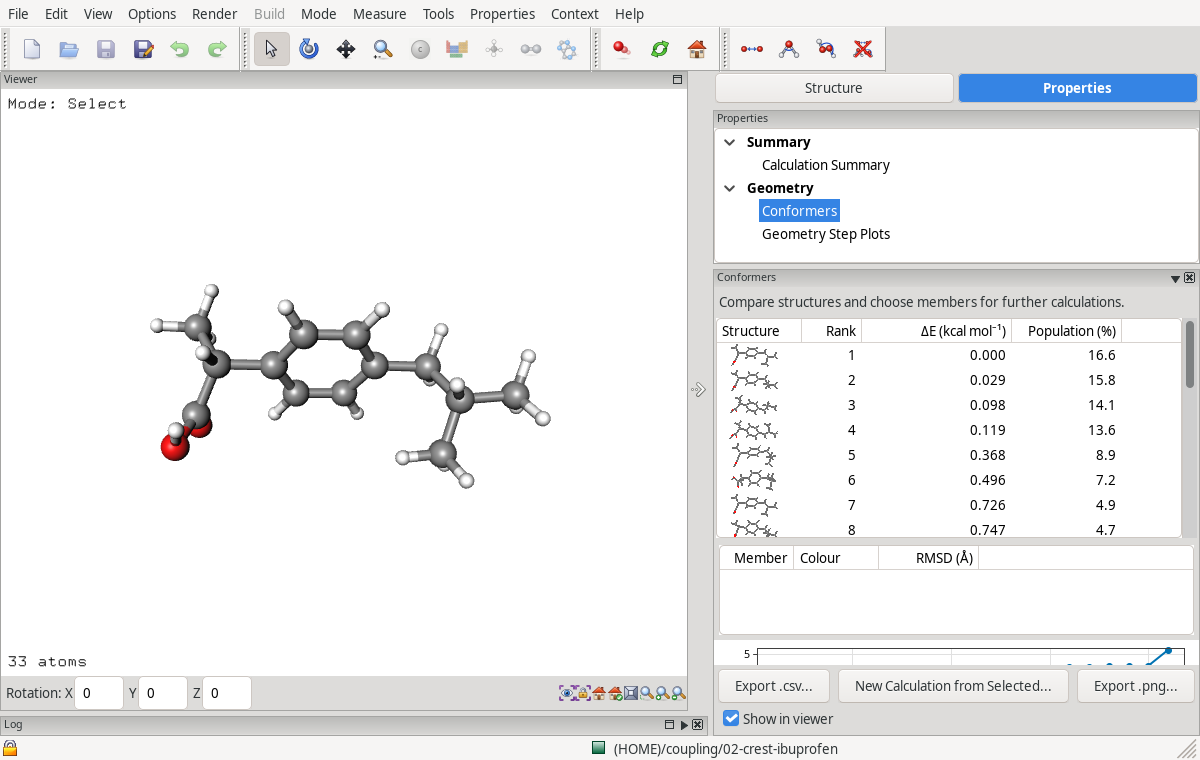
\includegraphics[width=\linewidth]{coupling/crest-conformers.ecce-9.5.3-dev.png}
	\caption{The \menu{Conformers} panel for the CREST search on ibuprofen. The rows give rank, relative energy and population within GFN-FF; the 3-D view shows the lowest conformer on a white background.}
	\label{fig:coupling-conformers}
\end{figure}

\subsection{xTB and the ranking}
Each of the eight picks was optimised with GFN2-xTB (\SIrange{33}{48}{\second} each) and then given a single-point energy with ORCA and r2SCAN-3c \cite{grimme2021} on the xTB structure (\SIrange{33}{102}{\second} on four cores), so that the order of the conformers at the three levels could be set side by side. Table~\ref{tab:coupling-rank} gives the order and, for each method, the energy relative to that method's own lowest conformer. The columns are not to be subtracted from one another.
\index{Ranking of conformers}

\begin{table}[htb]
	\centering
	\caption{Eight distinct conformers of ibuprofen at three levels. Each energy column is relative to the lowest conformer of that column, in kcal/mol; conformer 3 is the lowest at the xTB level and conformer 4 at the r2SCAN-3c level.}
	\label{tab:coupling-rank}
	\begin{tabular}{rrrrrrr}
		\toprule
		Conformer & \multicolumn{2}{c}{GFN-FF} & \multicolumn{2}{c}{GFN2-xTB} & \multicolumn{2}{c}{r2SCAN-3c} \\
		 & rank & rel. & rank & rel. & rank & rel. \\
		\midrule
		1 & 1 & 0.00 & 3 & 0.01 & 2 & 0.09 \\
		2 & 2 & 0.03 & 2 & 0.01 & 4 & 0.11 \\
		3 & 3 & 0.10 & 1 & 0.00 & 3 & 0.10 \\
		4 & 4 & 0.12 & 4 & 0.02 & 1 & 0.00 \\
		5 & 5 & 0.37 & 6 & 0.47 & 6 & 0.64 \\
		6 & 6 & 0.50 & 5 & 0.45 & 5 & 0.60 \\
		7 & 7 & 0.73 & 8 & 0.75 & 7 & 1.56 \\
		8 & 8 & 0.75 & 7 & 0.74 & 8 & 1.60 \\
		\bottomrule
	\end{tabular}
\end{table}

Inside each of three groups, conformers 1 to 4, 5 and 6, and 7 and 8, the order changes from one method to the next, and the differences within a group are a few hundredths of a kcal/mol at the xTB level and about a tenth at the r2SCAN-3c level, so the order inside a group has no meaning at any of the levels. The groups themselves keep their order at all three: the first four are always lowest, the pair 5 and 6 next, the pair 7 and 8 highest. This is the situation for which the funnel is designed. A cut at the lowest conformer of the cheap method would have dropped conformer 4, which the most expensive method puts first, and a cut after four conformers would have kept it. Passing on several conformers, and not one, costs a few minutes here.
\index{Funnel!choice of the number of structures}

The group structure is itself a result for ibuprofen: the four lowest conformers are separated from the rest by a gap that is larger than the differences inside them, and at the GFN-FF level the populations of all eight conformers are above 4 percent, so that a Boltzmann average over this molecule at room temperature would need more than the lowest one. Whether the gap persists at a higher level is a question for a calculation at that level and is not settled by this table.

\subsection{Refinement with ORCA}
The conformer that xTB put lowest, conformer 3, was optimised with r2SCAN-3c in ORCA from its xTB structure (Fig.~\ref{fig:coupling-orca}). The optimisation converged in 10 steps and \SI{341}{\second} on four cores, and moved the heavy atoms by \SI{0.096}{\angstrom} (RMSD after a fit). In the carboxyl group the C=O bond is \SI{1.201}{\angstrom} in the xTB structure and \SI{1.209}{\angstrom} after the optimisation, the C--O single bond \SI{1.340}{\angstrom} and \SI{1.357}{\angstrom}, and the O--H bond \SI{0.971}{\angstrom} in both. A step from tight-binding to a density functional therefore changes bond lengths by a few hundredths of an ångström and leaves the conformer as it was, which is what makes the hand-off of the structure sensible.
\index{Geometry optimisation!ORCA}\index{Bond lengths!carboxyl group}

\begin{figure}[htb]
	\centering
	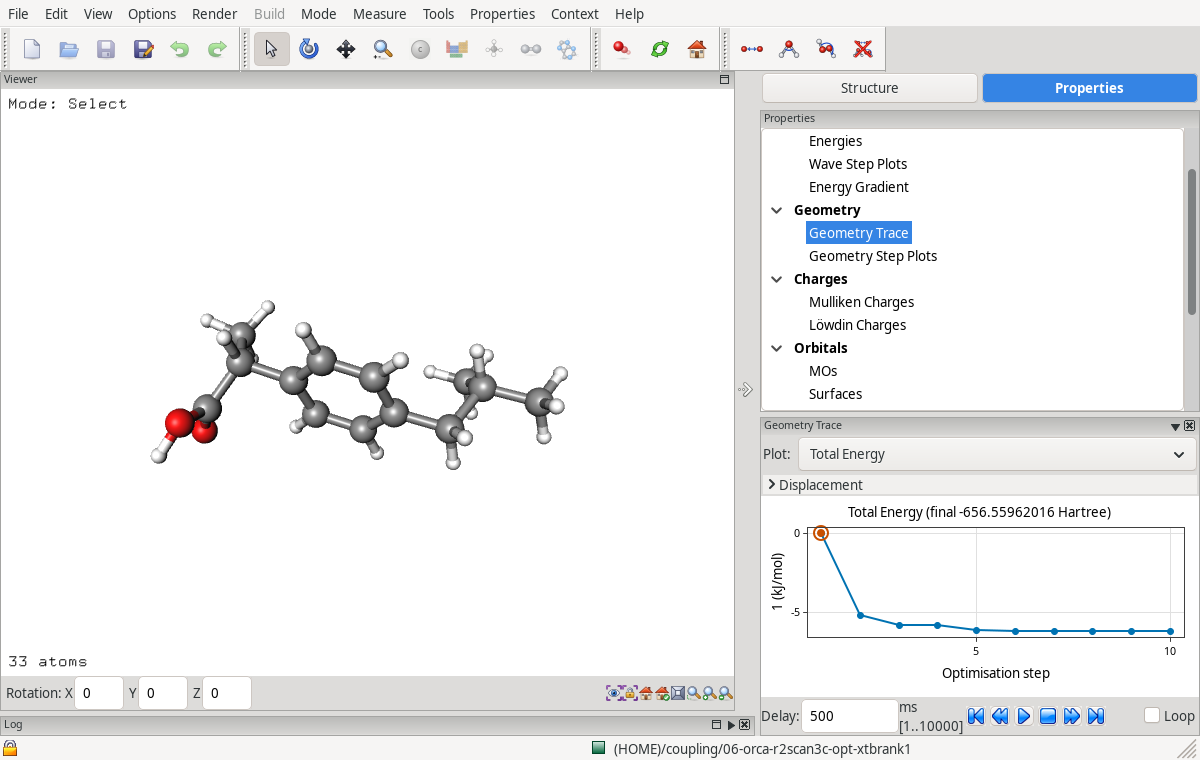
\includegraphics[width=\linewidth]{coupling/orca-opt-trace.ecce-9.5.3-dev.png}
	\caption{The ORCA r2SCAN-3c optimisation of ibuprofen conformer 3 in the Builder, with the \menu{Geometry Trace} panel plotting the energy of each optimisation step relative to the first.}
	\label{fig:coupling-orca}
\end{figure}

The calculations are in the repository of this book under \texttt{calculations/coupling}, in the order of the funnel: \texttt{01-xtb} the starting structure, \texttt{02-crest} the search, \texttt{03-xtb} the eight re-optimisations, \texttt{05-orca} the eight single points and \texttt{06-orca} the optimisation. A real project would stop earlier or later, depending on what the structure is wanted for. Frequencies and free energies, for instance, would be one more calculation on the last structure, in the same code, from \menu{New from This > Continue from Last Geometry}.
\index{New from This!Continue from Last Geometry}

\section{Across scales and from periodic models}
\index{Periodic models!to clusters}\index{Cluster models}

The hand-offs below were not run for this chapter. They are what the help pages of ECCE describe, and each is given with the page that describes it so that it can be checked against the version in use.

\emph{A periodic model into a cluster for a molecular code.} ECCE has no command that cuts a cluster out of a periodic structure and caps the cut bonds in one step. The pieces exist in the Builder: \menu{Edit > Select Within Distance...} selects the atoms, or whole molecules, within a distance of the current selection (with an option to keep the original selection), \menu{Edit > Reverse Selection} and \menu{Edit > Delete Selection} remove the rest, and the \menu{Delete Lattice} button of the Periodic Builder removes the cell. \menu{Build > Add Hydrogen} fills open valences from the atom shapes. That works for an organic fragment, but on a cut oxide every added atom needs checking. A new calculation then hands the cluster to a molecular code, for example through \cmd{ecce-series} with a template of that code. The user decides which atoms to keep and how to saturate the surface, and compares the cluster with the periodic model for the property of interest, not for the total energy.
\index{Select Within Distance}\index{Edit menu!Select Within Distance...}\index{Periodic Builder!Delete Lattice}\index{Edit menu!Delete Selection}\index{Edit menu!Reverse Selection}

\emph{A machine-learned potential into a quantum code.} A MACE calculation of a periodic cell or a molecule is cheap enough to optimise a structure first; the help page of the MLP code advises a Geometry run followed by a new calculation from its last structure for the property that needs a minimum. The same step, a new calculation in Quantum ESPRESSO or CP2K from the final geometry, is the hand-off from the machine-learned potential to the quantum code. Chapter~\ref{ch:mlp} describes the potential.
\index{MACE}\index{Codes!MACE}

\emph{Molecular dynamics and quantum chemistry.} A trajectory (a \texttt{.trj} or multi-frame \texttt{.xyz} file) opens in the Builder with \menu{File > Open...}, and a frame that is saved as a structure can be the source of a new calculation by the same route as above. \menu{Edit > Take Coordinates From...} puts the coordinates of chosen atoms of one calculation of the same folder into another that has the same atoms in the same order, with an optional alignment first, which is how a QM-optimised ligand is put back into a larger system.
\index{Take Coordinates From}\index{Trajectories!to quantum chemistry}

\section{One structure, each property from the best code}
\index{Properties!from different codes}

The last pattern needs no new mechanism. One structure, for instance the r2SCAN-3c structure of conformer 3 above, is the source of several calculations that differ in the code: the orbitals and a population analysis in ORCA, a vibrational spectrum from xTB or from ECCE-QM, a dipole moment or a surface from another code, each made from the same stored geometry by \cmd{ecce-series} or by the \menu{New step} window, so that the coordinates are exactly the same in each. Within one code, \menu{New from This > Continue from Final Orbitals} starts the new calculation from the orbitals of the finished one for ORCA, Gaussian 16, NWChem, ECCE-QM, MOPAC, CP2K and Quantum ESPRESSO, which saves iterations for a larger basis set.
\index{Continue from Final Orbitals}\index{Series of calculations}
What each code does best is a question for the chapters of the field in which the property matters. The only rule that the coupling itself adds is the one used in Table~\ref{tab:coupling-rank}: the properties of different codes are read side by side, as structures, orders and quantities of the same kind, and the total energies of different methods are not subtracted.

\section{Where next}
The chapters of the Organic part use the funnel from the CREST search onwards (Chapter~\ref{ch:crest}), and the Inorganic part adds the solvation shell and the counter ions (Chapter~\ref{ch:pom-solvation}). The Materials part takes the periodic route (Chapters~\ref{ch:cp2k}, \ref{ch:mlp} and~\ref{ch:crystals}) and the Biochemistry part the docking funnel (Chapter~\ref{ch:docking}). Chapter~\ref{ch:workflows} shows how to draw a chain once and launch it as a unit.
